\documentclass{article}
\usepackage[utf8]{inputenc}
\usepackage[francais]{babel}
\usepackage{lmodern}
\usepackage[a4paper, margin=3cm]{geometry}
\usepackage{fancyhdr}

%Package for math expression
\usepackage{amsmath}
\usepackage{cancel}
\usepackage{amsthm,amstext,amsfonts,bm,amssymb,amsthm}
\usepackage{bm}
\usepackage{gensymb}
\usepackage{mathrsfs}
\usepackage{physics}
\usepackage{nicefrac}
\usepackage{pgffor}

%Package for graphic expression
\usepackage{graphicx}
\usepackage{wrapfig}
\usepackage{float}
\usepackage{caption}
\usepackage{subcaption}
\usepackage{enumitem}
\usepackage{fancyhdr}
\usepackage{sectsty}
\usepackage{multirow}

\usepackage{mathtools}
\DeclarePairedDelimiter\ceil{\lceil}{\rceil}
\DeclarePairedDelimiter\floor{\lfloor}{\rfloor}

\usepackage{pgffor}

\DeclarePairedDelimiter\absol{\lvert}{\rvert}%

% Header
\pagestyle{fancy}
\fancyhf{}
\rhead{Éric Pfleiderer}
\fancyhead[L]{Problème à N-Corps: la matière sombre}
\chead{}
\rfoot{}
\cfoot{\thepage}

\begin{document}
	
\begin{titlepage}
	\centering
	\vspace*{1cm}
	\textsc{\LARGE Université de Montréal}\\[1cm] 
	\textsc{\Large PHY 3075 -- Modélisation Numérique en Physique}\\[3cm]
	\vspace{1cm}
	\rule{\linewidth}{0.5mm} \\[0.5cm]
	{\LARGE \bfseries Problème à N-corps: \\ La matière sombre} \\[0.2cm]
	\rule{\linewidth}{0.5mm} \\[3cm]
	\vspace{1cm}
	\large par: \\*
	Éric Pfleiderer \\* 
	20048976\\[3cm] 
	\vspace{1cm}
	{\large \today}\\[3cm]
	\vfill
\end{titlepage}

\section*{Résumé}\label{sec:resume}

L'objectif de ce laboratoire est caractériser le comportement d'un système à $N$ corps lorsqu'en présence d'un halo de matière sombre. Plus précisément, on cherche à trouver une ou plusieurs combinaisons de paramètres définissant un halo qui mène à une courbe de rotation plate en fonction de la distance de l'origine. On cherche aussi à comparer l'étendu spatiale et la masse du halo à celle du système de particules. On trouve initialement deux combinaisons valides de paramètres, soit les vecteurs solutions $v_{sol}=(\sigma_0=1.5\times 10^8, r_H=21.3, \alpha=9.9$) et $v_{sol}=(\sigma_0=1.84\times 10^8, r_H=33.2, \alpha=8.63$). Par contre, la masse des halos associés à ces paramètres ne représente qu'une petite fraction de celle du système de particules, tandis que leurs étendues spatiales sont similaires. Lorsqu'on cherche un halo qui mène à une courbe de rotation plate mais qui possède aussi une masse importante, on trouve le vecteur solution $v_{sol}=(\sigma_0=2.16\times 10^9, r_H=54.37, \alpha=21.40$). Le halo associé possède un étendu spatiale plusieurs fois celui du système de particules.

\section{Introduction}\label{sec:introduction}

La matière sombre est une forme de matière hypothétique qui serait responsable pour la grande majorité de la masse dans l'univers. Son existence serait nécessaire à l'explication de plusieurs phénomènes, entres autres des phénomènes gravitationnelles qui resteraient inexpliqués si seul la matière visible était présente. Mais qu'en est-il du rôle de la matière sombre dans la formation des galaxies? Est-elle nécessaire à la formation de galaxies spirales? Engendre-t-elle des comportements uniques?

Le but principale de ce laboratoire est de simuler un système à $N$ corps interagisseant gravitationnellement et d'imposer la présence d'un halo de matière sombre afin d'étudier son effet sur le système. On désire plus spécifiquement décrire le type de halo qui produit une courbe de rotation plate en fonction de la distance de l'origine; comment sa masse se compare-t-elle à celle de la galaxie? Le halo et la galaxie ont-ils une étendue spatiale similaire? 


\section{Théorie}\label{sec:theorie}

Le problème à $N$ corps consiste à résoudre les équations du mouvement de $N$ particules interagissant ensemble à partir de leur position et vitesse initiale. Dans notre cas, on s'intéresse au mouvement d'étoiles interagissant gravitationnellement dans un puit de potentiel; on tente de simuler une galaxie spirale similaire à la Voie lactée.

Le mouvement des particules dans le système peut être décrit à l'aide du champs gravitationnel ainsi que des conditions initiales. Ce champs gravitationnel implique la présence d'un champs de potentiel qui est obtenu par l'intégrale volumique \ref{eq:potential_integral}, où on intègre la densité massique et on normalise par la distance entre la contribution et le point de mesure. Pour $N$ corps, on doit donc effectuer et sommer $N$ de ces intégrales, ou encore définir $V$ comme le volume joint de tous les corps.

\begin{equation}\label{eq:potential_integral}
	\phi(r) = - \int_{V} \frac{G \sigma_{tot}(r')}{\norm{r-r'}}dV'
\end{equation}

Dans le cadre de ce laboratoire, on inclut une contribution à la densité $\sigma_{tot}$ provenant d'un halo de matière sombre décrit par l'équation \ref{eq:density_DM}. L'intégrale \ref{eq:potential_integral} prend alors la forme plus explicite \ref{eq:potential_integral_DM}, où $\sigma$ représente la densité surfacique attribuée à la présence de particules et $\sigma_H$ représente la densité surfacique attribuée au halo.

\begin{equation}\label{eq:density_DM}
	\sigma_H(r) = \frac{\sigma_0}{1+(\nicefrac{r}{r_H})^{\alpha}}
\end{equation}

\begin{equation}\label{eq:potential_integral_DM}
	\phi(r) = - \int_{V} \frac{G (\sigma(r') + \sigma_H(r'))}{\norm{r-r'}}dV'
\end{equation}

Une fois un champs de potentiel $\phi(r)$ défini, il est possible de définir expicitement le champs de force gravitationnel \textbf{F} qu'on peut utiliser pour la résolution des équations de mouvement. Ce champs de force est décrit par l'équation \ref{eq:force}, qui stipule que la force en tout point de l'espace est proportionnelle au gradient du potentiel gravitationnel en ce point. 

\begin{equation}\label{eq:force}
	\textbf{F} = - \nabla \phi
\end{equation}

Finalement, on peut s'intéresser aux conditions d'équilibre dy système en invoquant la troisième loi de Kepler (voir \ref{eq:kepler}). En supposant que la force centrifuge est égale à la force gravitationnelle, on déduit la vitesse angulaire $\omega$ nécessaire pour observer un orbite circulaire. On utilise ces conditions d'équilibre comme conditions initiales du systèmes.

\begin{equation}\label{eq:kepler}
m r \omega^2 = \frac{GmM}{r^2} \Longleftrightarrow \omega = \sqrt{\frac{GM}{r^3}}
\end{equation}

\section{Méthodologie}\label{sec:methodologie}

\subsection{Modélisation numérique}\label{subsec:modelisation_numerique}

On définit un domaine d'étude $X \times Y$ tel que $X, Y \in [-L, L]$, dans lequel on place $N$ corps de masse $m$. Les positions initiales des planètes sont générées selon une distribution gaussienne $ G \sim (0, r_d)$. Les unités employées au cours de l'expérience sont affichées au tableau \ref{tab:units}.

\begin{table}[H]
	\centering
	\begin{tabular}{|c|c|c|}
		\hline
		Quantité & Unité choisies & Unité Internationales\\
		\hline
		Masse (m) & Masse solaire & $1.99\times10^{20}$\ kg\\ 
		Longueur (L) & KiloParsec & $3.086\times10^{19}$\ m\\ 
		Temps (t) & Rotation galactique & $7.5 \times 10^{15}$\ s \\ 
		\hline
	\end{tabular}
	\caption{Choix d'unités employées durant l'ensemble du laboratoire, à moins de spécifications contraires}
	\label{tab:units}
\end{table}

Pour calculer le potentiel gravitationnel $\phi$, on subdivise d'abord le domaine étudié en $M \times M$ cellules et on pose les relations 

\begin{equation*}
x_k = (k+\nicefrac{1}{2}) \times \Delta, \hspace{1cm} y_l = (l +\nicefrac{1}{2}) \times \Delta, \hspace{1cm} k, l = 0, ..., M-1\ ,
\end{equation*}
où $\Delta = \nicefrac{2L}{M}$ est la taille d'une cellule. Pour chacune de ces cellules, on compte le nombre $n$ de corps inclus, on multiplie par la masse solaire et on divise par la surface, tel qu'indiqué à l'équation \ref{eq:density_M}, afin d'obtenir la densité surfacique. On ajoute aussi la contribution de la matière sombre via l'équation \ref{eq:density_DM}, s'il y a lieu.

\begin{equation}\label{eq:density_M}
\sigma(x_k, y_l) = \frac{n \times m}{\Delta^2}
\end{equation}

Similairement, on définit une grille de taille $(M+1) \times (M+1)$ et on pose les relations

\begin{equation*}
x_i = i \times \Delta, \hspace{1cm} y_j = j \times \Delta, \hspace{1cm} i, j = 0, ..., M\ .
\end{equation*}

Cette grille est décalée d'un demi $\Delta$ par rapport aux subdivisions du domaine et sert à calculer le potentiel gravitationel aux coins de chaque subdivision. La figure \ref{fig:double_grille} affiche un exemple d'un tel calcul, où la droite représente la distance entre une contribution au potentiel et le coin où le potentiel est calculé.

\begin{figure}[H]
	\centering
	\hspace{-1cm}
	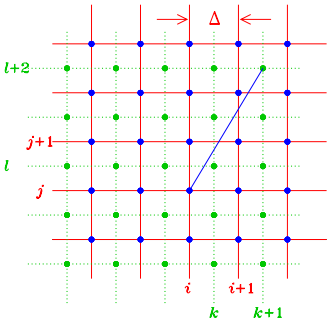
\includegraphics[scale=0.7]{images/doublegrid.PNG}
	\caption{Grille double utilisée pour le calcul du potentiel gravitationnel. Les indices $(i, j)$ représentent la grille du calcul de potentiel, alors que les indices $(k, l)$ représentent la grille du calcul de densité surfacique. \cite{notes_cours}}
	\label{fig:double_grille}
\end{figure}

Numériquement, l'intégrale \ref{eq:potential_integral} pour le calcul du pontentiel en un point devient une double somme, tel qu'indiqué à l'équation \ref{eq:potential_doublesum}. Le calcul du potentiel pour l'ensemble du domaine est donc de l'ordre de $\sim \Theta (M^4)$; la définition de la résolution spatiale via le paramètre $M$ doit donc être restreinte par soucis du temps de calcul. 

\begin{equation}\label{eq:potential_doublesum}
\phi(x_i, y_i) = - \sum_{k=0}^{M-1} \sum_{l=0}^{M-1} \frac{G \sigma (x_k, y_l)}{\sqrt{(x_i-x_k)^2+(y_j-y_l)^2}} \Delta^2
\end{equation}

Finalement, on applique l'algorithme de \textit{Verlet} (voir \ref{eq:verlet}) pour passer à la prochaine étape de la simulation; la première étape de l'algorithme consiste à mettre à jour les positions des corps, tandis que la deuxième consiste à mettre à jour leur accélération et la dernière, leur vitesse. On impose des conditions limites qui simulent des collisions élastiques lorsque les corps \textit{frappent} les frontières du domaine étudié. Les dérivées sont calculées numériquement par différence finie et centrée.

\begin{equation}\label{eq:verlet}
	\begin{gathered}
	x^{n+1} = x^n + v_x(\Delta t) + \frac{1}{2}a_x^n (\Delta t)^2\\
	y^{n+1} = y^n + v_y(\Delta t) + \frac{1}{2}a_y^n (\Delta t)^2\\
	\\
	a_x^{n+1} = \frac{-1}{m} \frac{\partial \phi}{\partial x}\\
	a_y^{n+1} = \frac{-1}{m} \frac{\partial \phi}{\partial y}\\
	\\
	v_x^{n+1} = v_x^n + \frac{\Delta t}{2} (a_x^n + a_x^{n+1})\\
	v_y^{n+1} = v_y^n + \frac{\Delta t}{2} (a_y^n + a_y^{n+1})
	\end{gathered}
\end{equation}

\subsection{Descente stochastique du gradient}

Notre objectif principal est de caractériser l'effet d'un halo de matière sombre sur un système à $N$ corps. Entre autres, on cherche une ou plusieurs combinaisons des paramètres $\sigma_0$, $r_H$ et $\alpha$ qui mènent à une courbe de rotation plate en fonction de la distance de l'origine. On quantifie donc l'allure de la courbe de rotation par une régression linéaire (voir \ref{eq:reg_lin}). 

\begin{equation}\label{eq:reg_lin}
	Y = \beta_0 + \beta_1 X + \epsilon
\end{equation}

On tente de minimiser la valeur absolue de la pente de la régression linéaire, tel qu'indiqué à l'équation \ref{eq:min_beta1}, tout en tentant de conserver une confiance élevée dans le modèle à travers son coefficient de détermination $R^2$.

\begin{equation}\label{eq:min_beta1}
	min\ \absol{\beta_1} = \absol{\frac{Y - \beta_0 - \epsilon}{X}}
\end{equation}

L'optimisation de la fonction (\ref{eq:min_beta1}) est effectuée par descente stochastique du gradient de type Monte Carlo. L'algorithme débute avec un vecteur solution initial $v_{sol} = (\sigma_0, r_H, \alpha)$ ainsi qu'une taille de pas caractéristique $h_i$ associée à chaque composante. Une série de piges aléatoires provenant d'une distribution normale (\ref{eq:pige_normale}) sont alors éffectués pour chaque composante du vecteur solution. 

\begin{equation}\label{eq:pige_normale}
	piges\ \sim G(\mu=0, \sigma=h_i)
\end{equation}

Les piges stochastiques sont ensuite sommées au vecteur solution original afin d'en obtenir un nouveau. Si le nouveau vecteur optimise davantage la fonction (\ref{eq:min_beta1}), il est maintenu pour la prochaine itération de la descente du gradient. Sinon, les piges sont poursuivis jusqu'à l'obtention d'une meilleur solution ou jusqu'à la rencontre d'un critère d'arrêt. Si de nombreuses piges sont effectués sans succès, on réduit les pas $h_i$ par un facteur $c=1/2$ afin de faciliter la convergence. Il est à noter que les descentes du gradient partagent une vulnérabilité avec un grand nombre de techniques d'optimisation; la convergence vers un minimum absolu n'est pas garantie. Le minimum choisi par la descente dépend des piges stochastiques, mais aussi grandement du vecteur solution initial, qui doit être choisi avec considérations. La descente stochastique peut aussi être répétée plusieurs fois avec le même vecteur solution initial pour tenter d'explorer une plus grande partie de l'espace des paramètres. L'implémentation de la descente stochastique employée dans le cadre de ce laboratoire est disponible sur le dépôt GitHub de l'auteur \cite{github}. Elle est basée sur le développement théorique introduit dans le manuel de notes \cite{notes_cours_phy1234}.

\section{Résultats}\label{sec:resultat}

\subsection{Effondrement gravitationnel}\label{subsec:effondrement}

À fins de validation du fonctionnement de l'algorithme de Verlet, on commence par simuler un système dont ont connait déjà le comportement. On initialise le système en imposant aux étoiles des vitesses intiales nulles et en les distribuant selon une loi gaussienne centrée en $\mu=0$ et dotée d'un écart-type de $r_H=6$. Sous ces conditions, une symétrie radiale apparaît lorsque $N \rightarrow \infty$ et garantie une force gravitationnelle dirigée vers l'origine. Cette symétrie est préservée avec une haute fidélité dans nos simulations en raison du nombre important de particules; on s'attend donc à observer un effondrement gravitationnel du système. En se référant à la figure \ref{fig:collapse}, on peut observer l'évolution d'une telle simulation incluant $N=10^5$ étoiles. Le système s'effondre rapidement dans les premier moments de la simulation, suivit d'une expansion à front circulaire bien défini. On note le développement caractéristique de structures radiales dû aux erreurs numériques provenant principalement de la discrétisation du calcul de forces. 


\begin{figure}[H]
	\centering
	\foreach \x [evaluate=\x as \evalx using int(\x*250)] in {2, 4, 6, 8, 9, 10, 12, 14, 16}{
		\begin{subfigure}{.3\linewidth}
			\centering
			\includegraphics[scale=0.3]{images/collapse/GravitationalCollapse\x.png}
			\caption{t = \evalx}
		\end{subfigure}
	}
	\caption{Instantanées d'une simulation d'effondrement gravitationnel avec vitesses initiales nulles où on recalcule le potentiel à toutes les 10 étapes. La simulation inclut $N=10^5$ particules, un quadrillage de $M \times M=49 \times 49$, un pas de temps de $\Delta=0.0002$ et un écart-type de $r_D=6$ pour la distribution gaussienne des positions initiales. }
	\label{fig:collapse}
\end{figure}

\subsection{Équilibre képlérien}\label{subsec:rotation}

On s'intéresse ensuite à simuler un système à $N$ corps en lui imposant des conditions initiales qui se traduisent par un équilibre képlérien; on impose des orbites circulaires où la force centrifuge équivaut à la force gravitationelle. À la figure \ref{fig:rotate_without}, on remarque une rotation qui devient rapidement désordonnée et qui s'effondre, provoquant le développement de spirales plus tard dans la simulation. On observe une dispersion relativement élevée des particules autour des bras et de la concentration sphérique centrale de la galaxie. La figure \ref{fig:courbe_rot_without} montre la courbe de rotation pour la même simulation à l'itération 7000, qui suit approximativement une équilibre képlérienne.

\begin{figure}[H]
	\centering
	\foreach \x in {250, 1000, 2000, 3000, 4000, 4500, 5000, 6000, 7000}{
		\begin{subfigure}{.3\linewidth}
			\centering
			\includegraphics[scale=0.35]{images/galaxy/without/galaxie\x.png}
			\caption{$t_I$ = \x}
		\end{subfigure}
	}
	\caption{Instantanées d'une simulation à orbites circulaires en équilibre képlérien où on recalcule le potentiel à toutes les 50 étapes. La simulation inclut $N=3\times 10^5$ particules, un quadrillage de $M \times M=65 \times 65$, un pas de temps de $\Delta=0.0002$ et un écart-type de $r_D=4$ pour la distribution gaussienne des positions initiales. Le temps $t_I$ est donnée ici en nombre d'itérations.}
	\label{fig:rotate_without}
\end{figure}

\begin{figure}[H]
	\centering
	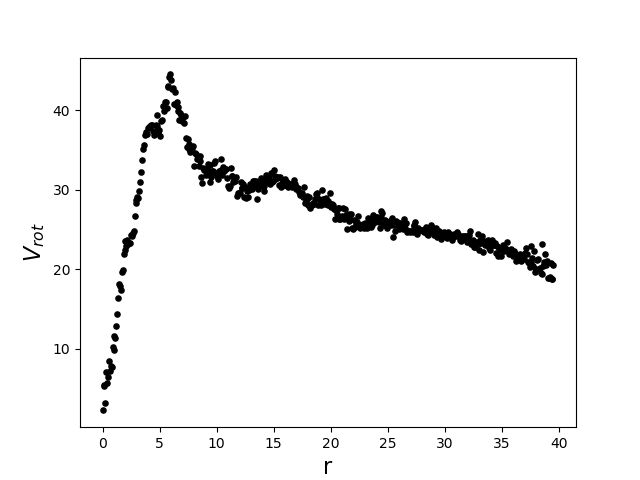
\includegraphics[scale=0.7]{images/VROTkepler.png}
	\caption{Vitesse moyenne de rotation en fonction de la distance de l'origine dans les phases finales de la simulation de la figure \ref{fig:courbe_rot_without}. La courbe représente approximativement un équilibre képlérien.}
	\label{fig:courbe_rot_without}
\end{figure}

\subsection{Recherche des paramètres optimaux}\label{subsec:parametres}

On s'intéresse ensuite aux combinaisons de paramètres $\sigma_0$, $r_H$ et $\alpha$ qui conduisent à une courbe de rotation demeurant plate en fonction de la distance du centre. Pour guider notre descente stochastique du gradient, on doit choisir un vecteur initial $v_{sol}$. On affine notre choix de $v_{sol}$ en se référant à la figure \ref{fig:etude_sigma} en annexe, qui montre l'impact des paramètres $\sigma_0$, $r_H$ et $\alpha$ sur la densité $\sigma_H$. À la figure \ref{subfig:r_H}, on remarque qu'une variation du paramètre $r_H$ engendre une translation de $\sigma_H(r)$ similaire à la propagation d'un front. À la figure \ref{subfig:alpha}, on observe un applanissement de la courbe lorsque $\alpha$ demeure bas. Inversément, $\sigma_H(r)$ se comporte comme un segment d'une fonction escalier lorsque $\alpha \rightarrow \infty$. Finalement, la figure \ref{subfig:sigma_0} montre simplement l'effet d'une constante multiplicative. De plus, on constate un point commun entre les trois figures; la densité surfacique atteint la moitier de sa valeur maximale au point $r=r_H$, ou encore $\sigma_H(r=r_H)=\frac{1}{2}\sigma_H^{max}$. Sous ces considérations, on choisit une solution initiale $v_{sol}=(\sigma_0=2\times 10^8, r_H=25, \alpha=5$). Les résultats de deux descentes du gradient sont consolidés au tableau \ref{tab:param}.

\begin{table}[H]
	\begin{center}
		\caption{Paramètres amenant une courbe de rotation plate en fonction de la distance de l'origine. On compte 5 itérations pour la descente du gradient et 5 itérations Monte Carlo. Les incertitudes proviennent de la taille des pas associé à chaque composante du vecteur $v_{sol}$ à la fin de la descente du gradient.}
		\label{tab:param}
		\begin{tabular}{|c|c|c|} % <-- Alignments: 1st column left, 2nd middle and 3rd right, with vertical lines in between
			\hline
			\textbf{$r_H$} & \textbf{$\sigma_0  (\times 10^8)$} & \textbf{$\alpha$} \\\hline
			$21.3 \pm 0.1$ & $1.5 \pm 0.2$ & $9.9 \pm 0.1$\\
			$33.68 \pm 0.07$ & $1.8 \pm 0.1$ & $8.71 \pm 0.07$\\\hline
		\end{tabular}
	\end{center}
\end{table}

On explicite davantage les résultats du tableau \ref{tab:param} en affichant les courbes de rotation respectives aux figures \ref{fig:courbe_rot_opt1} et \ref{fig:courbe_rot_opt2} ainsi que des instantanées à la figure \ref{fig:rotate_with} en annexe. En considérant les courbes de rotation, on constate que les pentes $\beta_1$ des régressions linéaires demeurent relativement plates, tel que recherché. Les régressions éffectués négligent l'intervalle où $r \leq 7.5$ afin d'augmenter la fiabilité du modèle.  On remarque que le coefficient de détermination varie grandement entre les deux solutions, ce qui implique que certains vecteur solutions sont plus prometteurs que d'autres; bien que la pente soit minimale à la figure \ref{fig:courbe_rot_opt2}, la faible valeur de $R^2$ se traduit par une faible valeur explicative du modèle. Inversément, le comportement de la courbe de la figure \ref{fig:courbe_rot_opt1} se rapproche beaucoup plus d'une droite, mais la pente demeure non-négligeable. Finalement, on remarque que les instantanées montrent une diminution de la dispersion des particules autour des bras de la galaxie comparativement à la figure \ref{fig:rotate_without}. Les structures qui se développent demeurent plus localisées lorsqu'en présence d'un halo.


% Ces résultats pourraient être expliqués par le grand temps de calcul nécessaire aux simulations qui se traduit par une plus faible exploration de l'espace des paramètres par la descente du gradient.

\begin{figure}[H]
	\centering
	\includegraphics[scale=0.7]{images/optimized/VROTOptimized1a.png}
	\caption{Courbe de rotation de la simulation choisie par la descente du gradient. La valeur des paramètres ainsi que les valeurs associés à la régression linéaire sont affichés. On termine les simulations dans les phases finales de la simulation, vers $t\approx 1.5$.}
	\label{fig:courbe_rot_opt1}
\end{figure}

\begin{figure}[H]
	\centering
	\includegraphics[scale=0.7]{images/optimized/VROTOptimized2a.png}
	\caption{Courbe de rotation de la simulation choisie par la descente du gradient. La valeur des paramètres ainsi que les valeurs associés à la régression linéaire sont affichés. On termine les simulations dans les phases finales de la simulation, vers $t\approx 1.5$.}
	\label{fig:courbe_rot_opt2}
\end{figure}

On peut déterminer la masse totale du halo de matière sombre en intégrant sa densité massique sur sa surface tel que montré à l'équation \ref{eq:masse_halo}. Lorsqu'on calcule\footnote{Les intégrales sont résolues à l'aide du module \textit{integrate} de la libraire \textit{scipy} en Python} les masses $m_1$ et $m_2$ des deux halos de la table \ref{tab:param}, on remarque qu'ils ont presque deux ordres de grandeurs de différence avec la masse $m_{N}=10^{11}$ du système. Or, la contribution de la matière sombre est habituellement importante, voir dominante dans les systèmes galactiques. On conclut que des courbes de rotations plates sont possibles, mais que les conditions nécessaires à leur développement sont potentiellement rares ou inexistantes.  Additionnellement, on remarque que l'étendu spatiale du halo, principalement régit par le paramètre $r_H$ lorsque $\alpha$ est élevé, est similaire à l'étendu spatiale de la galaxie, qui termine la simulation avec un rayon approximatif de $r \approx 20$.

\begin{equation}\label{eq:masse_halo}
	m_{tot} = \int_S \sigma_H dS= \int_{0}^{\infty} \int_{0}^{2 \pi} \frac{\sigma_0}{1+(\nicefrac{r}{r_H})^{\alpha}} dr d\theta = 2 \pi \int_{0}^{\infty} \frac{\sigma_0}{1+(\nicefrac{r}{r_H})^{\alpha}} dr
\end{equation}

\begin{equation}\label{eq:masse_halo1}
	m_{tot}^1 = 2 \pi \int_{0}^{\infty} \frac{1.5 \times 10^8}{1+(\nicefrac{r}{21.30})^{9.9}} dr \approx 3.33 \times 10^9
\end{equation}

\begin{equation}\label{eq:masse_halo2}
	m_{tot}^2 = 2 \pi \int_{0}^{\infty} \frac{1.8 \times 10^8}{1+(\nicefrac{r}{33.68})^{8.71}} dr \approx 6.16 \times 10^9
\end{equation}


On cherche maintenant à déterminer si les courbes de rotations plates sont possibles lorsque la contribution provenant du halo de matière sombre est de l'ordre de celle provenant du système de particules. On cherche une combinaison de paramètres $\sigma_0$, $r_H$ et $\alpha$ qui mène vers une courbe plate mais qui respecte aussi le ratio de masse typiquement observé dans la nature entre la matière sombre et la matière visible. On choisit le vecteur solution initial $v=(\sigma_0=2\times 10^9, r_H=50, \alpha=20$), qui se traduit par une masse environ équivalente au système de particule selon l'intégrale \ref{eq:masse_halo3}, et on lance une série de nouvelle descentes. Le résultat le plus prometteur est affiché à la figure \ref{fig:courbe_rot_opt3}.

\begin{equation}\label{eq:masse_halo3}
m_{tot}^3 = 2 \pi \int_{0}^{\infty} \frac{2 \times 10^9}{1+(\nicefrac{r}{50})^{20}} dr \approx 1 \times 10^{11}
\end{equation}
\begin{figure}[H]
	\centering
	\includegraphics[scale=0.7]{images/optimized/VROTOptimized3a.png}
	\caption{Courbe de rotation de la simulation choisie par la descente du gradient. La valeur des paramètres ainsi que les valeurs associés à la régression linéaire sont affichés. On termine les simulations dans les phases finales de la simulation, vers $t\approx 1.5$.}
	\label{fig:courbe_rot_opt3}
\end{figure}

On remarque une confiance élevée en la régression linéaire et une pente qui demeure non-négligeable. De plus, on voit que le rayon final du système de particules est $r \approx 12$, une diminution de presque $\nicefrac{1}{2}$ par rapport aux deux halos étudiés précédemment. De plus, les étendues spatiales ne sont plus comaparables; le halo termine la simulation avec un rayon qui est $\approx 5$ fois plus grand que celui du système.

Au final, on voit qu'il est possible d'engendrer des courbes de rotations avec des intervalles où la courbe est plate. Par contre, il est difficile de trouver une combinaison de paramètres optimaux se traduisant par une régression linéaire à faible pente et à haute confiance ($R^2$). Une explication possible serait la taille variable des systèmes de particules à la fin de la simulation; dépendamment de la masse du halo et de sa distribution, le système peut finir avec un rayon $\in [10,40]$. Il devient alors difficile de déterminer le sous-ensemble de points à employer dans la régression linéaire, ce qui diminue la précision de la descente du gradient. Une autre source importante de difficulté est le lourd temps de calcul nécessaire à une seule simulation, ce qui réduit considérablement le nombre d'itérations qu'on décide d'imposer à l'algorithme de descentente stochastique. Cette diminution dans le nombre d'itérations se traduit directement par une diminution de l'exploration de l'espace des paramètres formée par $r_H$, $\alpha$ et $\sigma_0$. Il devient alors difficile d'augmenter le nombre de résultats produits ou de les affiner. On conclut que la technique de descente du gradient n'est pas optimale dans ce contexte, à moins d'optimisation élevée du code afin de réduire son temps d'exécution ou à moins de paralléliser le calcul de sorte à opérer plusieurs recherches simultanément.

%\subsection{Conservation de l'énergie}\label{subsec:conservation}

\section*{Conclusion}

En simulant un système à $N$ corps massique interagisseant gravitationnellement, il a été possible d'étudier l'effet d'un halo de matière sombre sur un système galactique. Plus précisément, il a été possible de décrire les types de halos menant à une courbe de rotation plate en fonction de la distance de l'origine en employant une descente stochastique du gradient qui optimise la valeur absolue de la pente d'une régression linéaire. On trouve deux combinaisons de paramètres $\sigma_0$, $r_H$ et $\alpha$ qui produisent les courbes de rotation recherchées, soient les vecteurs solutions $v_{sol}=(\sigma_0=1.5\times 10^8, r_H=21.3, \alpha=9.9$) et $v_{sol}=(\sigma_0=1.84\times 10^8, r_H=33.2, \alpha=8.63$). Par contre, les halos représentés par ces vecteurs solutions ne concordent pas avec les observations typiques; leur masse totale ne forme qu'une faible fraction comparativement à la masse de la galaxie simulée. De plus, leur étendu spatiale est similaire à celle de la galaxie. Additionnellement, on conclut que l'efficacité de la méthode de recherche choisie, soit la descente stochastique du gradient, dépend fortement de l'optimisation et de la parallélisation du code employé.


\pagebreak

\section{Annexe}

\begin{figure}[H]
	\centering
	\begin{subfigure}{.7\linewidth}
		\centering
		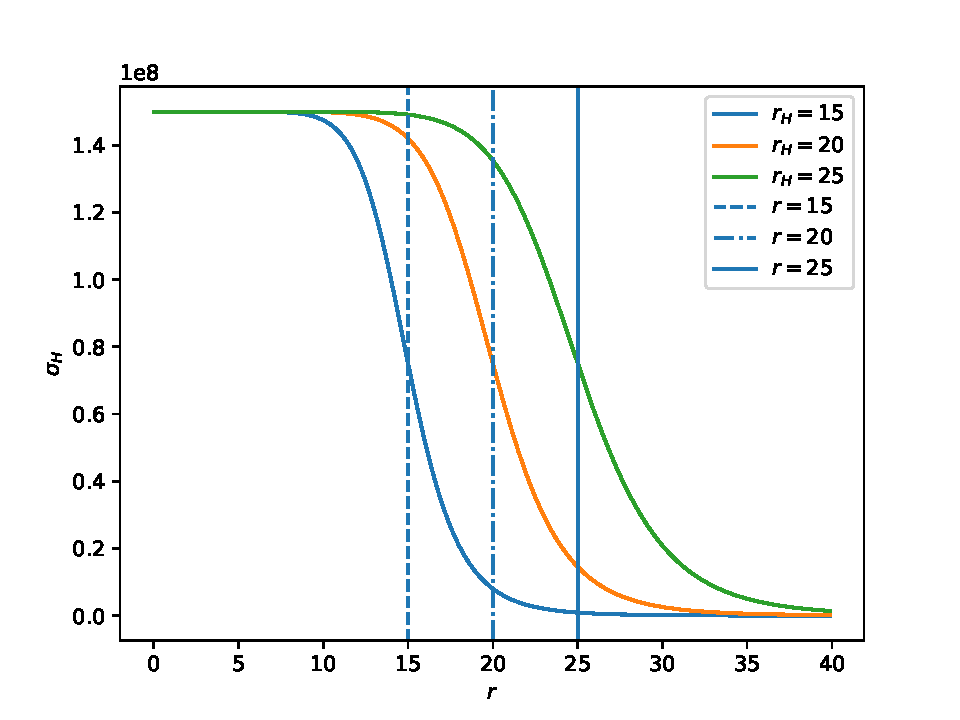
\includegraphics[scale=0.54]{images/sigma_r_H.pdf}
		\caption{Paramètre $r_H$}
		\label{subfig:r_H}
	\end{subfigure}
	\begin{subfigure}{.7\linewidth}
		\centering
		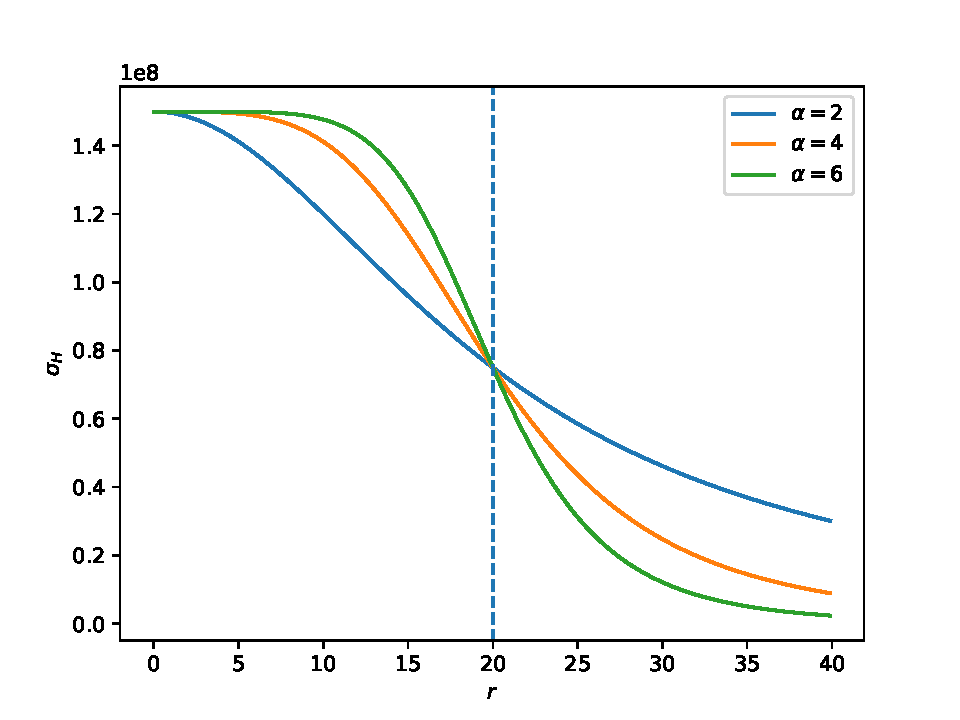
\includegraphics[scale=0.54]{images/sigma_alpha.pdf}
		\caption{Paramètre $\alpha$}
		\label{subfig:alpha}
	\end{subfigure}
	\begin{subfigure}{.7\linewidth}
		\centering
		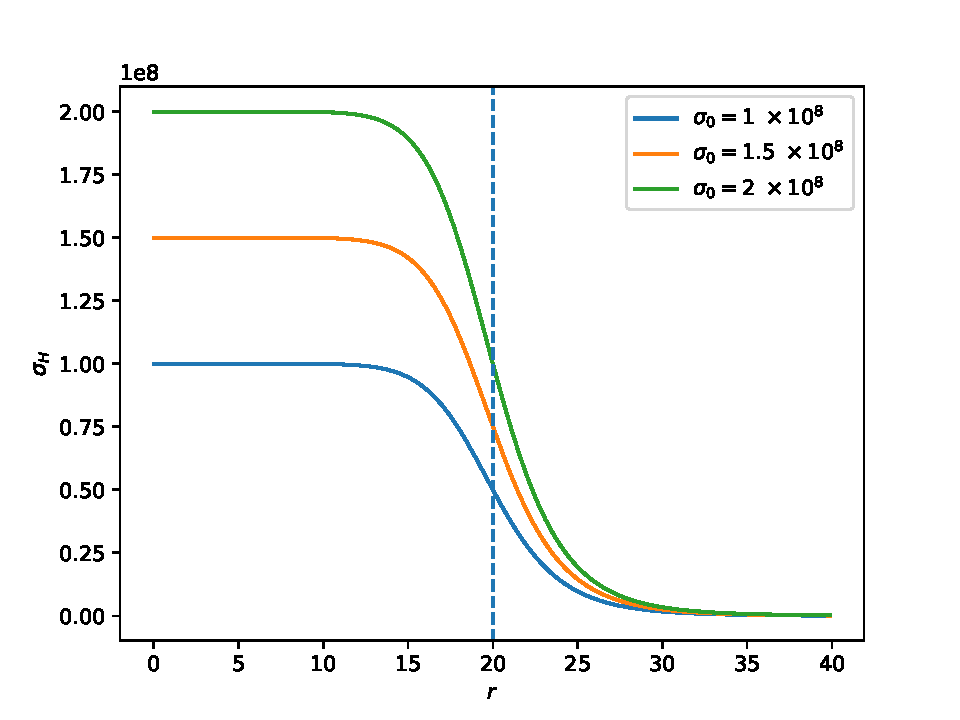
\includegraphics[scale=0.54]{images/sigma_sigma_0.pdf}
		\caption{Paramètre $\sigma_0$}
		\label{subfig:sigma_0}
	\end{subfigure}
	\caption{Variation de la densité surfacique $\sigma_H$ en fonction de la distance de l'origine. Chaque figure affiche trois courbes où on fait varier le même paramètre de courbe en courbe. Les intersections entre les courbes et les lignes verticales marquent l'endroit où $r = r_H$.}
	\label{fig:etude_sigma}
\end{figure}

\begin{figure}[H]
	\centering
	\foreach \x in {250, 1000, 2000, 3000, 4000, 4500, 5000, 6000, 7000}{
		\begin{subfigure}{.3\linewidth}
			\centering
			\includegraphics[scale=0.35]{images/galaxy/with/galaxie\x.png}
			\caption{t = \x}
		\end{subfigure}
	}
	\caption{Instantanées d'une simulation à orbites circulaires en présence d'un halo de matière sombre où on recalcule le potentiel à toutes les 50 étapes. La simulation inclu $N=3\times 10^5$ particules, un quadrillage de $M \times M=65 \times 65$, un pas de temps de $\Delta=0.0002$ et un écart-type de $r_D=4$ pour la distribution gaussienne des positions initiales. La valeur des paramètres $r_H$, $\alpha$ et $\sigma_0$ sont de $21.3$, $9.9$ et $1.5 \times 10^8$ respectivement.}
	\label{fig:rotate_with}
\end{figure}

\section{Bibliographie}\label{sec:bibliographie}
\begin{thebibliography}{l}
	\bibitem{notes_cours} 
	\textsc{Charbonneau}, P., Recueil de notes, Modélisation numérique en physique, Département de Physique, Université de Montréal, Janvier 2019
	
	\bibitem{notes_cours_phy1234} 
	\textsc{Charbonneau}, P., \textsc{Lafrenière}, D., Recueil de notes, Introduction à la physique numérique, Département de Physique, Université de Montréal, Automne 2016
	
	\bibitem{github}
	\textsc{Pfleiderer}, E., Dépôt GitHub, https://github.com/EricPfleiderer/Portfolio/tree/master/PHY3075/PROJET4
\end{thebibliography}


\end{document}